\chapter{Work Plan}
\lhead{\emph{Work Plan}}
(400 words)

The whole research project is divided into following work packages:
\begin{itemize}
\item WP 1 - Literature Review - 5 weeks - As part of this work package an additional literature review will be performed on the existing research conducted in the area of predictive bug detection as well as techniques available for building prediction models, be is as a big data analysis techniques or machine learning ones.
\item WP 2 - Problem Definition - 2 weeks - Based on the literature review adjust the definition of the research domain.
\item WP 3 - Building the infrastructure - 5 weeks - Acquisition and configuration of tools needed to conduct the research project including, but not exclusive to, data storage and analysis tools, supervised machine learning kits, configuring hardware and software for specific languages required as part of the research project, etc.
\item WP 4 - Data Gathering - 3 weeks - As part of this work package data necessary for building prediction as well as metrics for prediction model verification will be gathered for 2 microservice ecosystems. Both code metrics for training (X) and verification (Y) datasets will be gathered. Additionally, information about bugs reported for training set X will be collected. 
\item WP 5 - Data cleaning and processing - 4 weeks - The metrics, as well as bug reports for training set X, will be cleaned and bugs will be aligned to specific microservices they occurred in.
\item WP 6 - Building a prediction model - 10 weeks - As part of this work package a number of prediction model will be built using appropriate predictive algorithms, which will then be compared in terms of effectiveness. Then, the model will be tuned by adjusting the weighting of each metric for the prediction model as well as adjusting specific algorithm parameters influencing model accuracy.
\item WP 7 - Gathering data to verify prediction model - 4 weeks - The work package encompasses gathering, cleaning and aligning the bug reports for the verification dataset Y.
\item WP 8 - Verify prediction model - 6 weeks - As part of this work package the prediction model will be verified using dataset Y with conclusions drawn on the effectiveness of the model built.
\end{itemize}

\begin{figure}[h!]
\centering
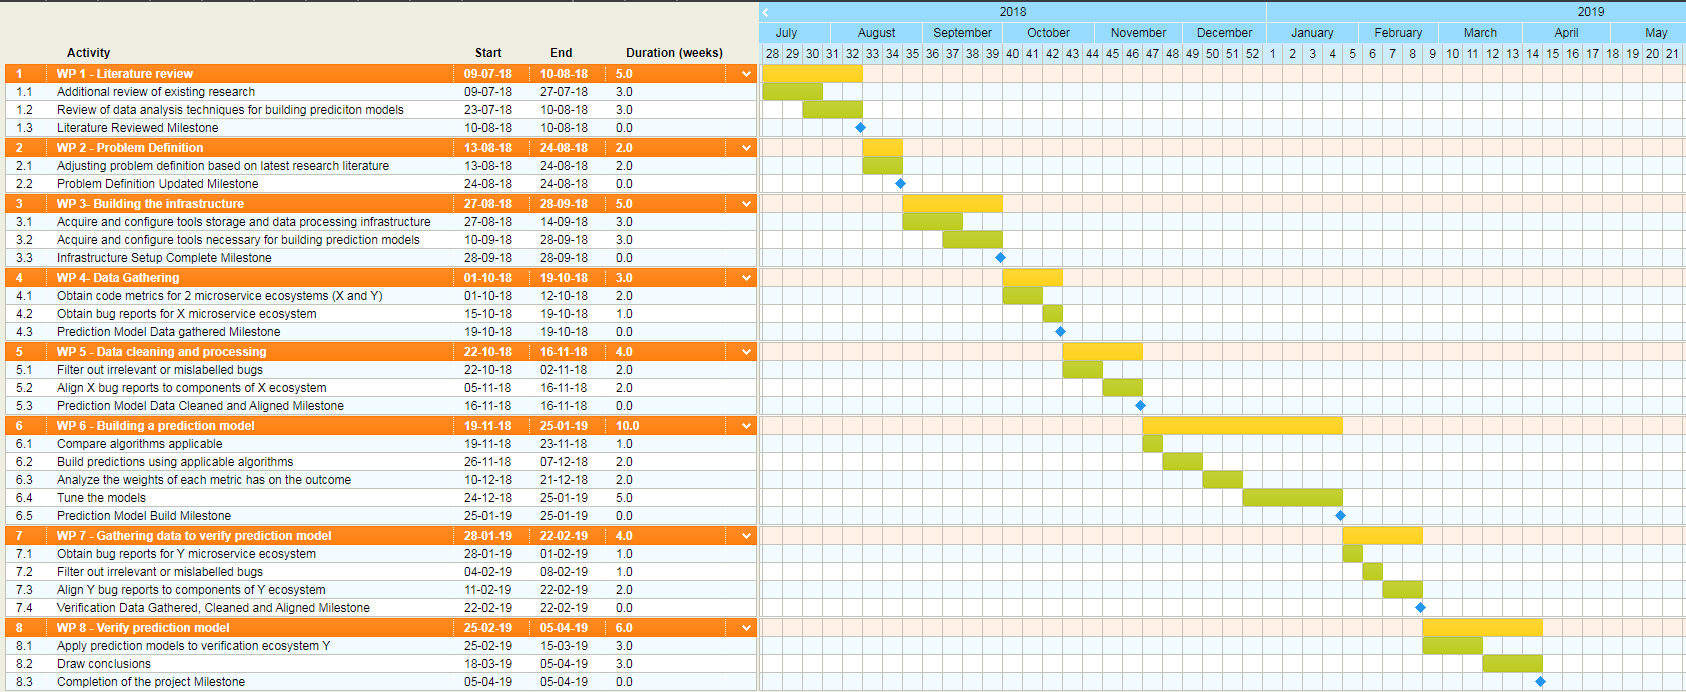
\includegraphics[width=1.0\textwidth]{Figures/Gantt_chart_final.png}
\caption{\label{fig:Actual Architecture}Project Schedule Gantt Chart}
\end{figure}

\begin{figure}[h!]
\centering
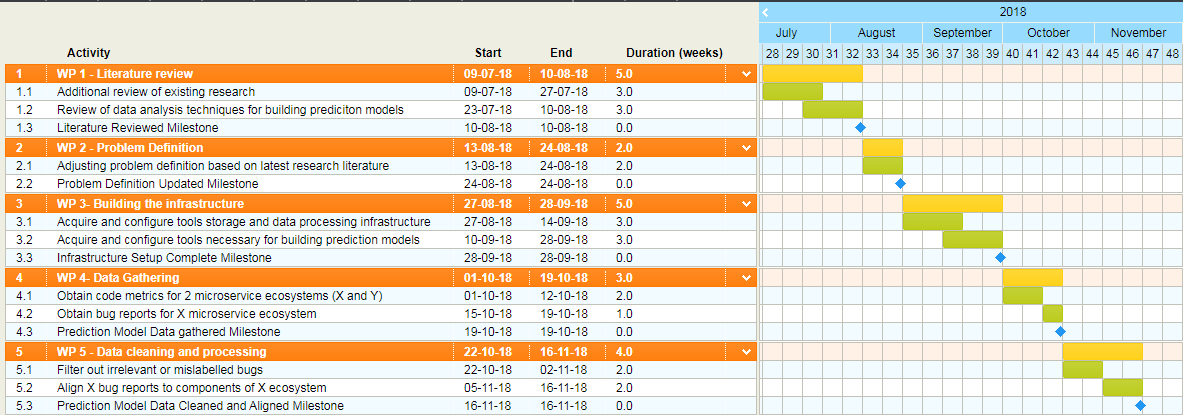
\includegraphics[width=1.0\textwidth]{Figures/Gantt_detail1.png}
\caption{\label{fig:Actual Architecture}Project Schedule Gantt Chart - Detail}
\end{figure}

\clearpage
\begin{figure}[h!]
\centering
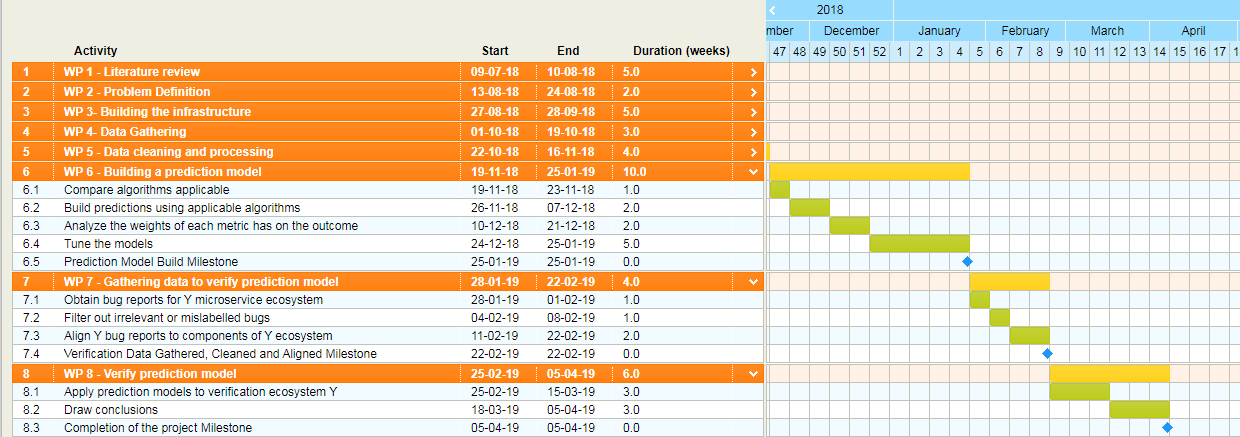
\includegraphics[width=1.0\textwidth]{Figures/Gantt_detail2.png}
\caption{\label{fig:Actual Architecture}Project Schedule Gantt Chart - Detail}
\end{figure}

The milestones set to be achieved through the above work packages are as follows:
\begin{enumerate}
\item Literature Reviewed
\item Problem Definition Updated
\item Infrastructure Setup Complete
\item Prediction Model Data gathered
\item Prediction Model Data Cleaned and Aligned
\item Prediction Model Build
\item Verification Data Gathered, Cleaned and Aligned Milestone
\item Completion of the project
\end{enumerate}